\chapter{Architecture}
\label{4}
\section{MAC Layer Architecture}
\begin{figure}[H]
\centering
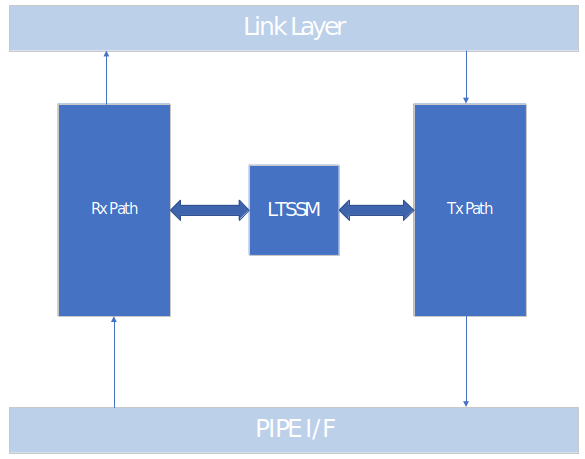
\includegraphics[width=130mm,height=130mm]{images/arch1.png}
\caption{MAC Layer Architecture}
  \label{fig:arch}
\end{figure}
Link Parameters:
  \begin{itemize}
    \item Number of Lanes: up to x16
    \item PIPE Width: up to 32
    \item Data Path: 512
    \item PIPE Per GEN
    \item The layer works on one clock which is the pclk.
  \end{itemize}
  \section{LTSSM Architecture}
\begin{figure}[H]
  \centering
  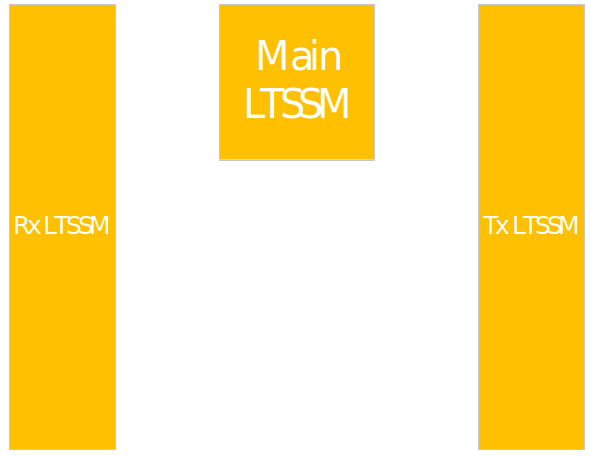
\includegraphics[width=100mm,height=100mm]{images/arch2.png}
  \caption{LTSSM Design}
    \label{fig:arch}
  \end{figure}
  LTSSM is divided into two main parts:
    \begin{itemize}
      \item Two substates :
      \begin{itemize}
        \item TX LTSSM
        \item RX LTSSM
      \end{itemize}  
      \item Main LTSSM : Represents spec states and Controls sub-states
    \end{itemize}
    
\section{TX Path Architecture}    
\begin{figure}[H]
  \centering
  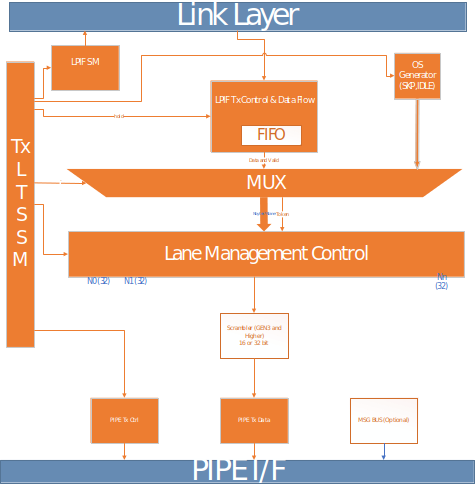
\includegraphics[width=130mm,height=130mm]{images/TX.png}
  \caption{TX Path}
    \label{fig:arch}
  \end{figure}
  Modules:
    \begin{itemize}
      \item Tx LTSSM : Controls all LTSSM functions for the Tx path.
      \item LPIF SM : Handles LPIF LTSSM.
      \item LPIF Tx Ctrl \& DF:
      \begin{itemize}
        \item Handles LPIF Interface.
        \item STP, SDP Generation.
        \item Data Valid Output.
      \end{itemize}
      \item OS Generator:
      \begin{itemize}
        \item Ordered Sets, Idle, SKP.
        \item Data Valid Output
      \end{itemize}
      \item MUX : multiplex between the data packets and ordered sets.
      \item Lane Management Control : perform byte Stripping on lanes.
      \item Scrambler.
      \item PIPE Tx Data
      \begin{itemize}
        \item Output data.
        \item Generate valid, sync header, start of block.
      \end{itemize}
      \item PIPE Tx Ctrl : Pclk handshake, pass rate, pclk rate, width, txdetectrx
      \item MSG BUS
    \end{itemize}
\section{RX Path Architecture}
  \begin{figure}[H]
    \centering
    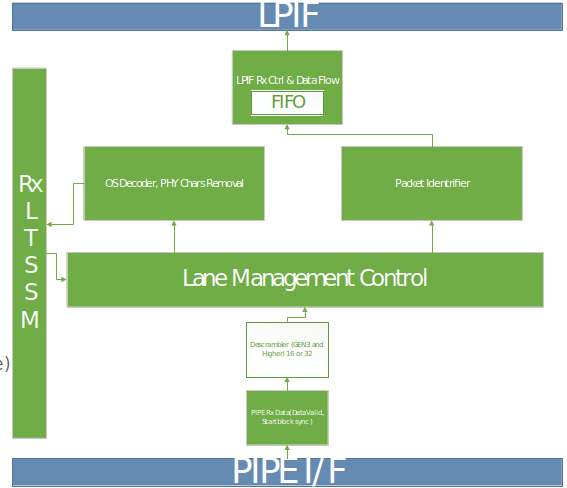
\includegraphics[width=130mm,height=130mm]{images/RX.png}
    \caption{RX Path}
      \label{fig:arch}
    \end{figure}
    RX modules:
      \begin{itemize}
        \item Rx LTSSM: Controls all LTSSM functions for the Rx path.
        \item PIPE Rx Data: Extract data wrt to header, valid, sb.
        \item Descrambler.
        \item LMC:
        Un stripe data no matter its type
        \item OS Decoder, Char Removal:
        \begin{itemize}
          \item Remove SKP, PAD, IDLE
          \item Decode TS and give data to LTSSM
        \end{itemize}  
        \item Packet Identifier:
        \begin{itemize}
          \item Remove STP, SDP and add sop, eop
          \item Forward packets only to Rx DF
        \end{itemize}
        \item LPIF Rx Ctrl \& DF:
        \begin{itemize}
        \item Forwards data to LPIF in 512 bit width (if applicable)
        \end{itemize}
      \end{itemize}